\section{Анализ предметной области}

\subsection{Базовые понятия и термины}
Прежде чем приступить к теме исследования, следует описать предмет исследования и связанные с ним термины.
В данной секции описаны понятия, которые будут использоваться в работе.

\subsubsection{Ядро Linux}
Ядро Linux — это основной компонент операционной системы Linux,
поскольку ядро отвечает за управление ресурсами компьютера и за взаимодействие приложений с аппаратными средствами.
Ядро должно в первую очередь выполнять две задачи:
\begin{enumerate}
    \item Взаимодействие с аппаратными компонентами, обслуживая низкоуровневые элементы, входящие в состав аппаратной платформы.
    \item Поддерживать среду выполнения для программ, которые будут выполняться в операционной системе.
\end{enumerate}

Для выполнения приведенных выше задач, ядро Linux реализует ряд архитектурных атрибутов.
Так, например, ядро разделено на отдельные подсистемы, каждый отвечающий за конкретные функции системы.
Примерами таких функций -- управление памятью, файловой системой, сетевыми интерфейсами, которые используются другими подсистемами.
Такое разделение упрощает разработку и поддержку ядра, а также увеличивает гибкость ОС.

Linux считается монолитной системой, поскольку все службы системы объединяются в одном цельном ядре,
что отличает данную концепцию от микроядерной архитектуры,
где каждая служба реализуется в отдельном модуле-ядре.
При запуске операционной системы ядро загружается в оперативную память компьютера и остается там до тех пор,
пока операционная система не будет выключена.
После того, как ядро загружено в оперативную память, ядро выполняет инициализацию и начинает планировать задачи.
Когда конкретная задача загружается, ей присваивается виртуальное адресное пространство, в котором будет пребывать.\vspace{0.5cm}\\

\indent Обобщая вышесказанное, можно сказать следующее:
ядро решает, какие ресурсы в каком порядке выделяются задаче для её выполнения.
В действительности же ядро действует как интерфейс между пользовательскими приложениями и оборудованием.\\
\indent Следует отметить, что не каждая задача получает равный доступ к ресурсам компьютера и подсистемам ядра,
поскольку в ином случае, например, при возникновении ошибки в одной из задач,
появляется шанс повредить как другие задачи, так и саму операционную систему.
Также следует понимать, что это далеко не единственная причина такого ограничения, однако,
чтобы понять, как ядро определяет к каким ресурсам и подсистемам процессы могут иметь доступ,
необходимо для начала представить модель загрузки задач в оперативную память.

\subsubsection{Виртуальная память}\label{subsec:-}

Виртуальная память --- это способ организации памяти, при котором процессору предоставляется не физические адреса, а виртуальные адреса, которые в дальнейшем переводятся в физические адреса с помощью таблиц страниц.
\\
Преимущество использования виртуальных адресов заключается в том,
что операционной системе становится доступно управление представлением памяти,
предоставляемой программному обеспечению.
На практике каждое приложение использует собственный набор виртуальных адресов,
которые будут отображаться в системе.
Каждый раз, когда операционная система переключается между приложениями, происходит перепрограммирование карты паммяти.
Это означает, что виртуальные адреса для текущего приложения будут сопоставлены с правильным физическим расположением в памяти~\cite{arm-virt}.\\
%Виртуальные адреса представляют собой набор бит, которые разбиваются на несколько частей: номер страницы, номер сегмента, номер региона\cite{virt-addressing} и номер суперстраницы\cite{superpage}.

\begin{figure}[H]
    \centering
    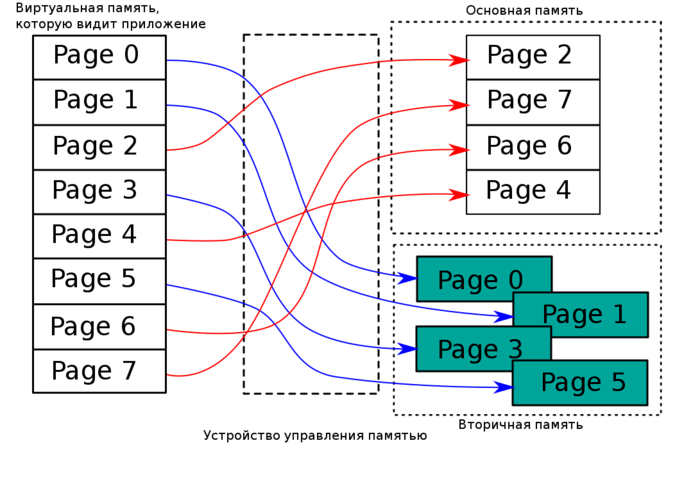
\includegraphics[scale=0.5,width=\textwidth]{inc/img/virt_mem}
    \caption{Схема устройства виртуальной памяти~\cite{virt-mem-pic}.}
    \label{fig:virt_mem}
\end{figure}

% \newpage

Помимо прочего, для виртуальной памяти разработаны инструменты для защиты памяти от несанкционированного доступа.
Виртуальная память распределяется на страницы с фиксированным размером, которые далее распределяются между процессами.
В случае, если процесс попытается получить доступ к странице, которая не принадлежит ему, то процессор сгенерирует исключение, которое будет обработано операционной системой.
\\
\indent Ввиду этого факта, виртуальная память приобретает важное дополнительное свойство.
Различные программы могут быть запущены в отдельных изолированных областях памяти, где они имеют доступ только к тем областям данным,
которые им необходимы для работы.
Отсюда мы переходим к появлению важного двух важных понятий: пространство ядра и пространство пользователя.
\newpage
\subsubsection{Пространство ядра и пространство пользователя}\label{subsec:----}
% FIXME?
Современные операционные системы, в частности Linux, разделяют виртуальную память на пространство ядра и пространство пользователя.
В пространство ядра помещаются само ядро и необходимые для работы модули.
Пространство пользователя в свою очередь разделяется на несколько частей.
Каждый процесс получает собственное пространство виртуальной памяти, в котором хранятся его данные, стек и куча.
Как было сказано выше, процессы в пространстве пользователя не имеют доступа к чужим областям памяти, однако такой возможностью обладают процессы запущенные в пространстве ядра, которые имеют доступ ко всем областям памяти.
Впервые данная концепция появилась в системе Multics, которая включала в себя 8 <<колец защиты>>\footnotemark, однако в UNIX-системах де-факто используются только два: кольцо 0 - отвечающее за ядро, и кольцо 3 - отвечающее за пользовательские приложения.
Кольца 1 и 2, предоставляемые некоторыми архитектурами процессоров, такие как x86, показали себя неэффективными ввиду сложности портирования на различные архитектуры процессоров, а также ряда других причин.
\\
Схематично данная концепция представлено на рисунке~\ref{fig:rings}.

\footnotetext{
    Такие архитектуры процессоров, как Intel x86, переняли эту концепцию и предоставляют 4 кольца защиты на уровне процессора, однако на практике 1-ое и 2-ое кольца практически нигде не используются.}

\begin{figure}[H]
    \centering
    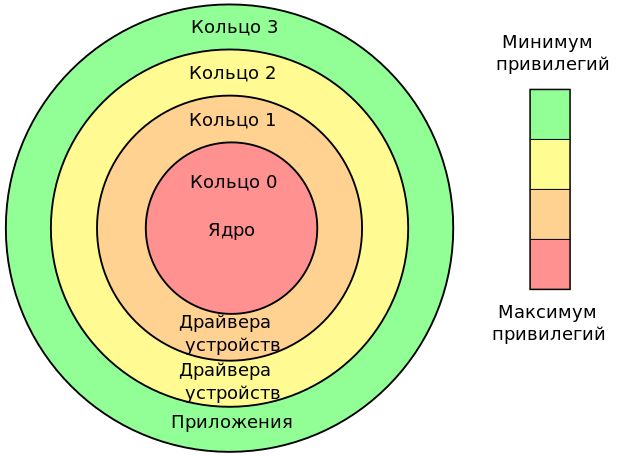
\includegraphics[scale=0.5,width=\textwidth]{inc/img/rings}
    \caption{Кольца защиты~\cite{rings-pic}.}
    \label{fig:rings}
\end{figure}

% \newpage
% FIXME?

Идея колец защиты заключается в том, что каждое кольцо имеет собственный набор инструкций, которые процесс на данном кольце защиты может выполнять, и чем ближе кольцо к нулевому, тем больше прав имеет процесс.
Однако поскольку в UNIX-системах используются только два кольца, то далее в работе будем к ним относиться как к пространству ядра и пространству пользователя для 0-го и 3-го колец соответственно, пренебрегая остальными.

\subsection{Способы модификации ядра Linux}\label{sec:--anal--methods}

В данной секции будет обозначено, что подразумевается под модификацией ядра Linux для определения в дальнейшем того, какие методы модификации ядра Linux существуют.

\subsubsection{Модификация ядра Linux}\label{subsec:--anal--methods--mod}

В данном разделе описаны критерии модификации ядра Linux.

\begin{itemize}
    \item[$-$] \textbf{Модификация ядра Linux} $-$ это изменение кода ядра Linux, которое не включает в себя изменение структуры ядра Linux.
    Таким образом программист волен изменять части ядра Linux, не затрагивая саму структуру ядра.
    Изменения, которые включают в себя изменение структуры ядра Linux, называются \textbf{переписыванием ядра Linux}, что выходит за рамки данного исследования.
    \item[$-$] Главное отличительная особенность модификаций ядра от других программ заключается в том, что работа модификаций происходит в пространстве ядра.
    Дополнительный функционал, который добавляется в ядро Linux, оперирует существующими структурами ядра Linux или создает собственные без ограничений со стороны ОС.
    \item[$-$] Модификации ядра имеют доступ ко всему функционалу ядра Linux, включая системные вызовы, обмен данными с устройствами и т.д.
    \item[$-$] Также модификации ядра манипулируют в любой области памяти, что позволяет взаимодействовать с другими модификациями ядра или самим ядром.
\end{itemize}

\subsubsection{Задачи модификации ядра Linux}\label{subsec:---linux}
%  FIXME?
Конкретные задачи модификации ядра крайне обширны и во многом зависят от конкретно поставленной цели конкретного проекта.
Вычисления на уровне ядра дают ряд преимуществ, такие как прямой доступ к оборудованию системы,
ускорение работы программы за счет отсутствия необходимости переключения между пространствами,
манипуляция данными в любой области памяти и т.д.
Однако для большого количества случаев такие преимущества либо не являются необходимыми, либо недостатки таких подходов нивелируют эти преимущества.
Общее правило, которое может быть сформировано для всех методов модификации ядра, выглядит следующим образом:
\begin{itemize}
    \item[$-$] Если вычисления на уровне ядра не являются необходимыми, то они не должны быть реализованы.
    \item[$-$] Если вычисления на уровне ядра все же являются необходимыми, то следует провести тщательный анализ, соизмеримое по времени с написанием программы, на тему того, нет ли других альтернатив.
    \item[$-$] Только в том случае, если вычисления на уровне ядра являются необходимыми и других альтернатив не существует, то с особой осторожностью можно приступить к написанию таких программ.
\end{itemize}

Другими словами можно сказать следующее: модификация ядра Linux должна быть последним вариантом,
когда остальные варианты исчерпали себя.
\\
\indent Следующий список дает примеры некоторых задач, которые должны быть решены на уровне ядра, однако ни в коей мере он не является полным или не лишенным исключений:
%FIXME?
\begin{enumerate}
    \item Написание приложений, таких как драйвера устройств, с доступом к низкоуровневым ресурсам, которые не могут быть предоставлены другими способами.
    \item Реализация алгоритмов, которые должны быть выполнены с высокой точностью по времени и/или пространству (например, мониторинг ресурсов системы или совместное использование ресурсов)~\cite{overhead-timer}.
    \item Написание программ, которые должны быть доступны всем пользователям системы~\cite{overhead-timer}.
    \item Также следует перейти в пространство ядра, где накладные расходы, такие как смена пространств пользователь-ядро, становится неприемлемыми для эффективной или корректной работы программы~\cite{overhead-timer}.
    Чаще всего в таких случаях речь идет об облачных вычислениях~\cite{overhead-cloud} или любых других вычислениях, требующих высокой производительности.
\end{enumerate}
